\part{Preliminaries}

\chapter{Significance of this thesis}
\minitoc
Nowadays, chaos is sometimes considered as the third scientific revolution of XXth century, after the relativity theory and the quantum mechanics~\cite{Pulch20121477}. In 1963, American meteorologist Lorenz found random behavior in some well-defined systems, and he proposed the ``butterfly'' theory, which broken Laplace determinism~\cite{begining_chaos}. In 1975, T.Y. Li and J. Yorke from Maryland University published a paper named ``period 3 implies chaos''~\cite{liyorke1975}, in which chaos was first used to reveal the process that how the order turns into disorder. 
As a surprising branch in natural science, chaos theory was formulated during the `60s and established in `70s. It is a blanketing theory that covers all aspects of science, such as mathematics~\cite{Pulch20121477, Elnashaie20073295, Chen20117258}, physics~\cite{Tian1997128,Chotorlishvili2010103}, biology~\cite{Yu2004341,Su12231}, chemistry~\cite{ElSayed2013148,Wu2009632}, and engineering~\cite{Lee199671,Aihara2012199}, etc.~\cite{Wu20104363,Du20092493}. Some researchers have pointed out that there exists tight relationship between chaos and randomness~\cite{Sunada2012190,Gon1999109}. So it is a natural idea to use chaos to enrich the design of new RNGs (Random Number Generators). In addition, since many chaotic systems have been extensively studied in past years, there are plenty of theoretical results that can be used to make performance analyses on the designed chaotic RNG. 



\section{History of Chaotic RNG}
Actually, the use of chaos in the realization of random numbers generators has been proposed and analyzed since many years~\cite{kellert1994wake, Eckhardt87, liyorke1975, Wu20051195,gleick2011chaos,gleick2011chaos}. John von Neumann suggested the use of logistic map in 1947~\cite{Eckhardt87}, partly because it had a known algebraic distribution, and its iterated values could be easily transformed into any desired distribution. Then, Robert A. J. Matthews proposed to generate binary sequences based on a generalized logistic map~\cite{Matthews:1984:DLE:67071.67073} in 1989. From then
on, digital chaotic RNGs attract more and more attention of many researchers
from different areas. Many different chaotic systems have been used: Logistic map \cite{ethesis69,ethesis74}, and its generalized version \cite{Matthews:1984:DLE:67071.67073}, 2-D Henon attractor \cite{ethesis67,ethesis95}, Chebyshev map \cite{ethesis75}, piecewise linear chaotic maps \cite{ethesis22,ethesis117}, and so on. Besides using chaotic maps,  in particular, discrete-time chaotic circuit have also been served as random sources in many chaos-based random number generators, such as
p-adic discrete-time chaotic systems \cite{ethesis86}, first-order non-uniformly sampling DPLL (Digital Phase-Locked Loop) circuits \cite{ethesis61}, etc.

Traditionally, the entropy source for a RNG is a physical random phenomena. Such sources of randomness
include  noise in resistors \cite{Cohen1988113}, phase noise of lasers \cite{Gay2001197}, radioactive decay \cite{Opendak1994570}, are the favorite entropy sources to generate ideal random numbers. However, the rates for these true random numbers are lower than 20 Mbits/s. Fortunately, due to the development of modern technology, nonlinear dynamics
in optics (laser dynamics, large delay optical, or optoelectronic cavities) with high complexity dynamics and speed are feasible~\cite{Larger2004609}. This is why many random number generators based on semiconductor lasers operating in chaos have been recently proposed~\cite{fast,ultrafast2009,ultrafast2010}.

    
\section{Motivation}
Most of chaotic RNGs originate from physics. Their state $s$ is a real in the interval  $[0 , 1]$, their output bit is computed as a function of the state. In the simplest case, if $ s>0.5 $, then the output is 1, else the output is 0. When they are realized in digital computers with finite computing precision, despite the desirable mathematical properties of the chaotic functions, their use in floating point based implementations of RNGs raise some problems. Indeed restricting a chaotic system to a finite universe always causes various issues such as short cycle length, non-ideal distribution and correlation functions. However, RNGs based on chaotic iterations was initiated by constructing a chaotic system on the integers domain instead of the real numbers domain. The topological chaotic properties of the generator are shown by a 
rigorous framework. The design goal of these generators was to take advantage of the random-like properties of real valued chaotic maps and, at the same time, secure optimal cryptographic properties. From the above discussion, I believe that the research on chaotic iterations will be helpful to benefit the conventional cryptology and open a broader road to the design of good RNGs. 

Optical chaos was an exciting field of research in mid `80s, which has seen a recent resurgence, especially in the last 4 years, as chaotic waveforms for random number generation found a deep interest within the community of analogue broadband chaotic optical systems. In 2009, Reidler \emph{et al.} published a paper entitled ``An optical ultrafast random bit generator'' \cite{ultrafast2009}, in which they presented a physical system for a random number generator based on a chaotic semiconductor laser. This generator is claimed to reach potentially the extremely high rate of 300 Gb/s. With my supervisors, we reported on analyses and experiments of their method, which has led to a discussion recalled in the third part of this thesis, about the actual origin of the randomness as well as to the actually reachable bit rate. We have shown that the actual binary sequence randomness corresponds more to complex mixing of noisy components performed by digital post-processing operations, than to chaotic properties of 
the signal. We have also addressed the issue of a proper 
way to use chaotic motion in RNGs, which is shown to necessarily involve MSBs instead of the LSBs. Without this criteria, physical noise alone is enough to retrieve a random sequence. However, in that case deterministic chaos cannot be used, e.g., for PRNG synchronization, as it would be of interest if one would like for instance to implement physically the one-time pad (the truly RNG becoming the keystream to be used only once for a perfectly secure encryption). Different random bit sequences have been investigated in that context, both from experimental time series generated by a recently proposed chaotic optical phase generator as well as from numerical simulations.

\section{Objectives of this thesis}

\subsection{The local research context}

This thesis focuses on the use of chaotic dynamics from nonlinear optical devices or chaotic mathematical systems, for generating pseudorandom numbers. 
During this thesis, a link has been established between two research teams of the
FEMTO-ST Institute  
(Universit\'{e} de Franche-Comt\'{e}%~\cite{ufc}
), namely the AND team 
(Distributed Numerical Algorithms%~\cite{and}
) and the OPTO (Optoelectronics, Photonics, and Optical Telecommunications) one. 
During this thesis, these teams have worked in a complementary manner on the generation of pseudorandom numbers. 

Firstly, the AND team has recently proposed a novel family of pseudorandom numbers generators (algorithms) 
based on mathematical chaos.
%a tool called chaotic iterations.
A short summary of these researches is given thereafter.
%, which satisfy the Devaney's definition of chaos. The idea is to use two 
%possibly defective random number generators as inputs and to mix them using chaotic iterations.
%Due to topological properties owned by this mixing way, disorder induced by the inputs is enlarged and thus
%statistical performances are improved. 
%In more details, i
It has been firstly proven in~\cite{guyeux09,guyeux10} that chaotic iterations (CIs), a suitable tool for fast computing iterative algorithms, satisfies the topological chaos property, as it is defined by Devaney~\cite{Dev89}. Indeed, this PRNG has been obtained by combining chaotic iterations and two generators based on the logistic map in~\cite{wang2009}. The resulted PRNG shows better statistical properties than each individual component alone. Additionally, various chaos properties have been established. 
The advantage of having such chaotic dynamics for PRNGs lies, among other things, in their unpredictability character. These chaos properties, inherited from chaotic iterations, are not possessed by the two inputted generators. 
The team has shown that, in addition of being chaotic, this generator can pass the NIST battery of tests, widely considered as a comprehensive and stringent battery of tests for cryptographic applications~\cite{ANDREW2008}.
Then, in the papers~\cite{guyeuxTaiwan10,bgw10:ip}, the speed of the former PRNG has been improved,
among other things by replacing the two logistic maps by two XORshifts in \cite{guyeuxTaiwan10}, and ISAAC with XORshift in \cite{bgw10:ip}. Additionally, the first generator is able to pass DieHARD tests \cite{guyeuxTaiwan10}, whereas the second one can pass TestU01 \cite{bgw10:ip}.
In~\cite{wbg10:ip,bfgw11:ij}, which is an extension of~\cite{wang2009}, the team has improved the speed, security, and evaluation of the former generator and of its application in information hiding. Then, a comparative study between various generators has been carried out and statistical results have been improved. %Chaotic properties, statistical tests, and security analysis allow us to consider that this kind of generator has better characteristics and is capable to withstand attacks. 

In prior literature, the iteration function was only the vectorial Boolean negation. It is then judicious to investigate whether other functions may replace the vectorial negation in the above approach. 
This is why %In~\cite{bcgw11:ip}, we combined its own function and its own PRNGs to provide a new PRNG instance, and proposed 
a method using graphs with strongly connected components has been proposed in~\cite{bcgw11:ip} as a selection criterion for chaotic iteration functions. The approach developed along these lines solves this issue by providing a class of functions whose iterations are chaotic according to Devaney and such that resulting PRNG success statistical tests.
Then the vectorial Boolean negation has been used as a prototype, and explanations about how to modify the iteration function without deflating the good properties of the associated generator has been brought in~\cite{bfgw11:ip}. Simulation results and basic security analysis have finally been presented to evaluate the randomness of this new family of generators.



Secondly, in the OPTO side, the physical source of entropy is originating from a strongly deterministic 
process too using chaotic lasers \cite{weicker:pre12,PhysRevE.86.055201,PhysRevLett.107.034103}. Experiments have recently demonstrated
that such an optical chaos can mask $10$ Gb/s of a given data signal during
transmissions over an installed fiber optic link \cite{lavrov:jqe10}. 
An important objective of  the OPTO team is then to explore different 
physical approaches, as efficiently as possible (in terms of speed and quality of 
randomness), to extract pseudorandom number sequences from analog chaotic dynamics. 
The physical devices that generate such dynamics are available and accessible via existing routines 
developed by the team.
Final targeted applications are the production of optical fiber communications broadband secured by chaos.



\subsection{The objectives}


In view of the state of the art detailed above, the main objective of my thesis was to use chaotic dynamics for generating pseudorandom numbers in various contexts. In more details, the aims was to:

\begin{itemize}
\item Develop and implement various algorithms including Version 1 CI, Version 2 CI, Version 3 LUT CI, and Version 4 CI, and to compare their performances with software and hardware based systems to evaluate the randomness of this new family of pseudorandom generators. For illustration purposes, all the proposed PRNGs should be used in well-detailed cryptographic application.

\item Evaluate the contributions of noise and chaos in fast random bit sequences generated from broadband optoelectronic entropy sources. Ways to keep a deterministic origin in the optical generation 
of pseudorandomness must be regarded too. Finally, an appropriate road to mix chaotic iterations with optical chaotic laser could be investigated, in order to design proper random streams that can be synchronized and used for cryptography. 
\end{itemize}

\section{Contributions}

The scientific contribution during this thesis has two aspects, related either
to computer science or to optics, which are reported in the two parts that follow
the introducing part of this manuscript.

On the one hand, the first part contains developments and evaluations of various CI PRNGs methods. 
These generators are based on discrete chaotic iterations, which satisfy the well-respected 
Devaney's definition of chaos. New versions of this original family of generations have been 
introduced, studied, and experimented. 
All the CIPRNG family has been completely rethought, in order to implement it in FPGA architectures, 
which has led to a well-appreciated and large speed improvement. The contributions in this
computer science oriented part end by application examples of use in cryptography.

On the other hand, in the second part, we have participated to a deep analysis of 
both the origin of chaos and
the deterministic character of the chaos-based photonic RNGs proposed 
in~\cite{ultrafast2009, ultrafast2010}. Our analysis strongly suggest that
their method essentially exploits the noisy compound of the photonic signal, which
is always present in such signals, would it be with (chaos) or without (noise) 
deterministic motion. Using only the most significant bits (or equivalently the 1-bit 
ADC conversion) is, according to this contribution, the unique solution to make
such an optic-based PRNG as deterministic, and thus reproducible. 


This thesis has led to the submission and/or the publication of the following articles.
\subsection{Peer-reviewed International Journals}
\begin{itemize}
% {Revue internationale}
\item Jacques Bahi, Xiaole Fang, Christophe Guyeux, and Qianxue Wang (alphabetic order). Evaluating Quality of Chaotic pseudorandom Generators. Application to Information Hiding. IJAS, International Journal On Advances in Security, 4(1-2):118--130. 2011~\cite{bfgw11:ij}.
\end{itemize}

\begin{itemize}
\item Jacques Bahi, Xiaole Fang, Christophe Guyeux, and Laurent Larger (alphabetic order). FPGA Design For Pseudorandom Number Generator Based On Chaotic Iteration Used In Information Hiding Application. Applied Mathematic \& Information Science. Submitted in Jan. 2013 \cite{submit1}.
\end{itemize}

\begin{itemize}
\item Jacques Bahi, Xiaole Fang, Christophe Guyeux, and Qianxue Wang (alphabetic order). Assessment of the suitability of three chaotic iterations schemes based on XORshift Generator for application in the Internet security field. JNCA, Journal of Network and Computer Applications, accepted. To appear \cite{submit2}.
\end{itemize}

\begin{itemize}
\item Jacques Bahi, Xiaole Fang, Christophe Guyeux, and Qianxue Wang (alphabetic order). FPGA Acceleration of a Pseudorandom Number Generator based on Chaotic Iterations. Cryptography and Communications. submitted in Jan. 2013 \cite{submit3}.
\end{itemize}

\begin{itemize}
 \item Xiaole Fang, Benjamin Wetzel, Jean-Marc Merolla, John M. Dudley, Laurent Larger,
Christophe Guyeux, and Jacques M. Bahi. Noise and chaos contributions in fast
random bit sequence generated from broadband optoelectronic entropy sources. In
IEEE Transaction on Circuits and Systems. Submitted in Jan. 2013.
\cite{submit4}.
\end{itemize}



\subsection{Peer-reviewed International Conferences}
\begin{itemize}
% {Actes de conférences internationales sélectives}

\item Qianxue Wang, Jacques M. Bahi, Christophe Guyeux, and Xaole Fang. Randomness quality of CI chaotic generators. Application to internet security. In INTERNET'10. The 2nd Int. Conf. on Evolving Internet, pages 125--130, Valencia, Spain, September 2010. IEEE seccion ESPANIA. Best paper~\cite{wbg10:ip}.%ok

\item Jacques M. Bahi, Xiaole Fang, Christophe Guyeux, and Qianxue Wang (alphabetic order). On the design of a family of CI pseudorandom number generators. In WICOM'11, 7th Int. IEEE Conf. on Wireless Communications, Networking and Mobile Computing, Wuhan, China, pages 1--4, September 2011~\cite{bfgw11:ip}.%ok

\item Jacques Bahi, Xiaole Fang, and Christophe Guyeux (alphabetic order). An optimization technique on pseudorandom generators based on chaotic iterations. In INTERNET'2012, 4-th Int. Conf. on Evolving Internet, Venice, Italy, pages 31--36, June 2012~\cite{bfg12a:ip}.

\item Jacques Bahi, Xiaole Fang, and Christophe Guyeux (alphabetic order). State-of-the-art in Chaotic Iterations based pseudorandom numbers generators Application in Information Hiding. In IHTIAP'2012, 1-st Workshop on Information Hiding Techniques for Internet Anonymity and Privacy, Venice, Italy, pages 90--95, June 2012~\cite{bfg12b:ip}.
\end{itemize}

\section{Thesis Organization}
The remainder of this manuscript is divided in four parts, as detailed below.

This first part details the significance and background of this thesis. An overview of random numbers and theirs generators is provided. Some techniques to generate chaotic random number, based on physical sources or mathematical mapping functions, will be discussed too. The fundamental views and definitions of chaotic iterations are then summarized. After these materials, some existing test suites, such as NIST statistical test suite, 
DieHARD battery of tests, ENT test program, Comparative test parameters, and TestU01, which are commonly used to verify the randomness of a sequence, are also introduced. The FPGA platforms, on which the PRNG systems will be built on, are finally presented.

In Part~\ref{Pseudo Random Number Generator Based on Chaotic Iteration}, the developments and applications of  chaotic iterations (CI) based pseudorandom number generators are presented. Firstly, The basic definitions concerning CI and PRNGs are recalled in Chapter~\ref{Introduction}. Then, Chapter~\ref{Review of works} shows some famous pseudorandom number generators and two versions of generators based on CI. In the next chapter, firstly the statistical analysis of the CI methods for random number generators is summarized, and their strength and weakness are also commented, then by understanding the random-like dynamics of chaotic iterations, some novel developments and versions of CI based PRNGs are described in Chapter~\ref{CI dev}. In the following chapter, %~\ref{Statistical Tests for Randomness} 
 the evaluation and comparison between the proposed CI generators, using the most famous statistical tests, are shown. 
The state-of-the-art of chaotic iterations-based PRNGs is given in Chapter~\ref{State-of-the-art}.
As FPGA (Field-Programmable Gate Array) chips provide sufficient logic and storage elements on which complex algorithms can be built, this technology is then used to improve the speed and performance of our CI generators in Chapter~\ref{FPGA Acceleration of CIPRNGs}. Lastly, 
%we first propose simple applications of these generators for encryption and information hiding in Chapter~\ref{State-of-the-art}; then 
an application example and its evaluations regarding the CI technology are expressed in Chapter~\ref{Application Example}.

The third part of this manuscript focuses on optic aspects of pseudorandom number generation. It is firstly verified in Part~\ref{Optoelectronic Chaotic Laser} that to use the MSBs (Most Significant Bits, or equivalently $1$-bit ADC conversion) is the key to keep a deterministic chaotic laser information in generation of random bits. Secondly, the applications of chaotic iterations to optoelectronic chaotic signals, as described
thereafter, is investigated. In Chapter~\ref{chaotic laser introdution}, a brief introduction on random number generators based on photonic technique is given. Then, in Chapter~\ref{Noise And Chaos Contributions In Fast Random Bit Sequence Generated From Broadband Optoelectronic Entropy Sources}, a recently published method~\cite{ultrafast2009, ultrafast2010} using chaotic waveform for pseudorandom generation is reprocessed and analyzed, leading to the conclusion that LSBs are definitely a major hurdle for regenerating the initial random sequence. Finally, Chapter~\ref{CI Random Stream Generation Via Optoelectronic Chaotic Laser} shows two examples in adapting chaotic iterations to simulated chaotic waveform, leading to the generation of random sequences.

This manuscript is then concluded in Part~\ref{end con}, which provides a summary of the researches that have been realized
during this thesis, and discussions about possible future work in this area is finally provided.

\section{Abbreviations}
\begin{tabular}{ll}\toprule
\textbf{Abbreviation}& \textbf{Definition}\\\hline
\textbf{RNGs}& Random Number Generators\\
\textbf{TRNGs}& True Random Number Generators\\
\textbf{PRNG}& Pseudo Random Number Generator\\
\textbf{NIST}& National Institute of Standards and Technology\\
\textbf{VOD}&Video on Demand\\
\textbf{FPGA}& Field Programmable Gate Array\\ \bottomrule
\end{tabular}
 

\section{Mathematical Symbols}
\begin{tabular}{@{}c@{}@{}l@{}}
\textbf{Symbol} &\textbf{Meaning}\\
$\llbracket 1;\mathsf{N} \rrbracket$ & $\rightarrow\{1,2,\hdots,N\}$ \\
$S^{n}$ & $\rightarrow$ the $n^{th}$ term of a sequence $S=(S^{1},S^{2},\hdots)$ \\
$v_{i}$ & $\rightarrow$ the $i^{th}$ component of a vector: $v=(v_{1},v_{2},\hdots, v_n)$\\
$f^{k}$ & $\rightarrow$ $k^{th}$ composition of a function $f$ \\
$\emph{strategy}$~ & $\rightarrow$ a sequence which elements belong in $%
\llbracket 1;\mathsf{N} \rrbracket $ \\
$mod$ & $\rightarrow$ a modulo or remainder operator\\
$\mathbb{S}$ & $\rightarrow$ the set of all strategies \\
$\mathbf{C}_n^k$ & $\rightarrow$ the binomial coefficient ${n \choose k} = \frac{n!}{k!(n-k)!}$\\
$\oplus$ & $\rightarrow$ bitwise exclusive or \\
%& $\begin{array}{r@{\;}l}\ f^{k}=\underbrace{f\circ ...\circ f} \\ \ k\ \text{times}\end{array}$\\
$+$ & $\rightarrow$ the integer addition \\
$\ll \text{and} \gg$ & $\rightarrow$ the usual shift operators \\
$(\mathcal{X}, \text{d})$ & $\rightarrow$ a metric space  \\
$\lfloor x \rfloor$ & $\rightarrow$ returns the highest integer smaller than $x$  \\
$n!$ & $\rightarrow$ the factorial $n!=n\times(n-1)\times\dots\times1$\\
$\mathds{N}^{\ast }$ & $\rightarrow$ the set of positive integers \{1,2,3,...\}
\end{tabular}





\chapter{Research Background}
\label{General Notions}
\minitoc
This chapter, serving as the background of this thesis,  
is devoted to basic notations and terminologies in the fields of chaos theory and random numbers.

\section{The Mathematical Theory of Chaos}

\subsection{General Presentation}

Chaos theory studies the behavior of dynamical systems that are perfectly predictable, yet appear to be wildly amorphous and without meaningful. 
Chaotic systems are highly sensitive to initial conditions, 
which is popularly referred to as the butterfly effect. 
In other words, small differences in initial conditions (such as those due to rounding errors in numerical computation) yield widely diverging outcomes, 
rendering long-term prediction impossible in general \cite{kellert1994wake}. This happens even though these systems are deterministic, meaning that their future behavior is fully determined by their initial conditions, with no random elements involved \cite{kellert1994wake}. In other words, the deterministic nature of these systems does not make them predictable \cite{kellert1994wake,Werndl01032009}. This behavior is known as deterministic chaos, or simply chaos. It has been well-studied in mathematics and
physics, leading among other things to the well-established definition of Devaney
recalled thereafter.





\subsection{On Devaney's Definition of Chaos}

Consider a metric space $(\mathcal{X},d)$ and a continuous function $f:\mathcal{X}\longrightarrow \mathcal{X}$, for one-dimensional dynamical systems of the form:
\begin{equation}
x^0 \in \mathcal{X} \textrm{  and } \forall n \in \mathds{N}^*, x^n=f(x^{n-1}),
\label{Devaney}
\end{equation}
the following definition of chaotic behavior, formulated by Devaney~\cite{Dev89}, is widely accepted~\cite{bibtexwangqianxue}.

\begin{definition}
 A dynamical system of Form~(\ref{Devaney}) is said to be chaotic if the following conditions hold.
\begin{itemize}
\item Topological transitivity:

\begin{equation}
\forall U,V \textrm{ open sets of } \mathcal{X},~\exists k>0, f^k(U) \cap V \neq \varnothing .
\end{equation}

Intuitively, a topologically transitive map has points that eventually move under iteration from one arbitrarily small neighborhood to any other. Consequently, the dynamical system cannot be decomposed into two disjoint open sets that are invariant under the map. Note that if a map possesses a dense orbit, then it is clearly topologically transitive.
\item Density of periodic points in $\mathcal{X}$.

Let $P=\{p\in \mathcal{X}|\exists n \in \mathds{N}^{\ast}:f^n(p)=p\}$ the set of periodic points of $f$. Then $P$ is dense in $\mathcal{X}$:

\begin{equation}
 \overline{P}=\mathcal{X} .
\end{equation}

Density of periodic orbits means that every point in the space is approached arbitrarily closely by periodic orbits. Topologically mixing systems failing this condition may not display sensitivity to initial conditions presented below, and hence may not be chaotic.
\item Sensitive dependence on initial conditions:

$\exists \varepsilon>0,$ $\forall x \in \mathcal{X},$ $\forall \delta >0,$ $\exists y \in \mathcal{X},$ $\exists n \in \mathbb{N},$ $d(x,y)<\delta$ and $d\left(f^n(x),f^n(y)\right) \geqslant \varepsilon.$

Intuitively, a map possesses sensitive dependence on initial conditions if there exist points arbitrarily close to $x$ that eventually separate from $x$ by at least $\varepsilon$ under iteration of $f$. Not all points near $x$ need eventually separate from $x$ under iteration, but there must be at least one such point in every neighborhood of $x$. If a map possesses sensitive dependence on initial conditions, then for all practical purposes, the dynamics of the map defy numerical computation. Small errors in computation that are introduced by round-off may become magnified upon iteration. The results of numerical computation of an orbit, no matter how accurate, may bear no resemblance whatsoever with the real orbit.
\end{itemize}

\end{definition}

When $f$ is chaotic, then the system $(\mathcal{X}, f)$ is chaotic and quoting Devaney: ``it is unpredictable because of the sensitive dependence on initial conditions. It cannot be broken down or decomposed into two subsystems which do not interact because of topological transitivity. And, in the midst of this random behavior, we nevertheless have an element of regularity.'' Fundamentally different behaviors are consequently possible and occur in an unpredictable way.






\subsection{Chaotic iterations}
\label{subsection:Chaotic iterations}

Let us now introduce an example of a dynamical systems family that has
the potentiality to become chaotic, depending on the choice of the iteration 
function. This family is the basis of the PRNGs we have studied and
developed during this thesis~\cite{GuyeuxThese10,bibtexwangqianxue}.

\begin{definition}
\label{Chaotic iterations}
The set $\mathds{B}$ denoting $\{0,1\}$, let $f:\mathds{B}^{\mathsf{N}%
}\longrightarrow \mathds{B}^{\mathsf{N}}$ be an ``iteration'' function and $S\in \mathbb{S}
$ be a strategy. Then, the so-called \emph{chaotic iterations} are defined by~\cite{Robert1986}:

\begin{equation}
\left\{\begin{array}{l}
x^0\in \mathds{B}^{\mathsf{N}}, \\
\forall n\in \mathds{N}^{\ast },\forall i\in \llbracket1;\mathsf{N}\rrbracket%
,x_i^n=
\left\{
\begin{array}{ll}
x_i^{n-1} & \text{if}~S^n\neq i \\
f(x^{n-1})_{S^n}  & \text{if}~S^n=i.
\end{array} 
\right. 
\end{array}
\right.
\end{equation}
\end{definition}

In other words, at the $n^{th}$ iteration, only the $S^{n}-$th cell is
\textquotedblleft iterated\textquotedblright . Note that in a more general
formulation, $S^n$ can be a subset of components and $f(x^{n-1})_{S^{n}}$ can
be replaced by $f(x^{k})_{S^{n}}$, where $k < n$, describing for
example delays transmission. For the
general definition of such chaotic iterations, see, e.g.~\cite{Robert1986}.

Chaotic iterations generate a set of vectors;
they are defined by an initial state $x^{0}$, an iteration function $f$, and a chaotic strategy $S$~\cite{GuyeuxThese10,bibtexwangqianxue}.
These ``chaotic iterations'' can behave chaotically as defined by Devaney, 
depending on the choice of $f$~\cite{GuyeuxThese10}.
Furthermore, they are able to circumvent the problem of quantization
errors when implementing chaotic systems on computers, as explained
in the next section.


\subsection{Chaos Deflation when Computing}

In the past two decades, the use of chaotic systems in the 
computer science security field has become more and more frequent,
for instance when designing cryptosystems, PRNGs, or hash functions.
However, when chaotic systems are realized in digital computers with finite computing precision, it is doubtful whether or not they can still preserve the desired dynamics of the continuous chaotic systems. Because most dynamical properties of chaos are meaningful only when dynamical systems evolve in infinite sets, these properties may become useless, deceptive, or ambiguous when the phase space is highly quantized (i.e., latticed) with a finite computing precision. In other words, 
the related problem is the dynamical degradation of continuous chaotic systems 
when they are implemented in finite computing precision. 


When chaotic systems are realized in digital circuits or computers, the dynamical systems
will be discretized both spatially and temporally.
That is to say, they will become
discrete-time and discrete-value chaotic systems~\cite{MazrooeiSebdani2008628} defined in discrete time and spatial
lattice with finite elements. Their dynamical properties will be deeply different from the properties of continuous-value systems and some dynamical degradation will arise, such as short cycle length and decayed distribution. This phenomenon has been reported and analyzed in various situations~\cite{Binder1986,Wheeler1989,Palmore1990,Blank1997,Li2005}.



The quantization errors, which are introduced 
at each iteration of digital chaotic systems on finite
state machines, 
make that ``pseudo orbits'' depart from real ones in
a very complex and uncontrolled manner. Due to the sensitivity of chaotic systems on initial conditions, even ``trivial'' changes of computer arithmetic can definitely change the pseudo orbits' structures.
Although all quantization errors are quite deterministic 
when the finite precision and the arithmetic are fixed, 
it is technically impossible to deal with these
errors. Some random perturbation models have been proposed to depict quantization errors in digital chaotic systems, but they cannot exactly predict the actual dynamics of studied digital chaotic systems and have been criticized because of their essentially deficiencies


To sum up, continuous chaos may collapse into the digital world, and the deflation of chaotic properties is hard
to measure or control when implementing chaotic
continuous systems on computers.
In that context, previous theoretical and practical
studies directed by the AND team have concluded to
the possibility to cope with this problem using 
chaotic iterations~\cite{GuyeuxThese10,bibtexwangqianxue}. 
This thesis is an additional building block in that
direction.



After having introduced the mathematical approach for describing 
chaotic dynamics together with an important example, we now roughly present
the optical understanding of this multifaceted notion.

\subsection{Optical Chaos}

Optical chaos, in this manuscript, will refer to chaos generated by laser instabilities using different schemes provided by semiconductors and fiber lasers. This optical chaos is observed in many non-linear optical systems.
It as been successfully applied in a cryptographic
context, for securing exchanges through optic fiber 
using optical chaos~\cite{Larger2004609}.
At this point, we can remark that:
\begin{itemize}
\item these systems are, of course, intrinsically dedicated to modern communication using optical fibers;
\item the dynamical processes involved in optical systems can be very fast, thus resulting in another interesting feature of chaos-based optical cryptosystems, their potentially very high encryption speed;
\item high complexity chaotic dynamics are obtained, whether due to intrinsic complex nonlinear coupling between light and matter interactions in lasers, or due to the presence of a large delay feedback cavity enabling dynamics with large number of degrees of freedom.
\end{itemize}

These chaotic dynamical systems will be used for 
pseudorandom number generation, this is why we 
introduce the context of such generations in the
next section. 

\section{General Presentation of (Pseudo)Random Generation}

A random number generator (RNG) is a computational or physical device designed to generate a sequence of numbers or symbols that lack any pattern. As its name indicates, it appears random.

It is always a difficult task to generate good random number/sequence. Although it is accepted that rolling a dice
is random, such a mechanical method is not 
usable in practice, at least for the applications we
intend to consider. 
In past decades, random numbers were usually  generated offline, based on some dedicated setup or devices, and the sequences were stored in tables ready for use. These random tables are still available in the world-wide-web or some data CDROMs.
However, due to online requirements and security issues, random tables have recently become inappropriate, and hence different ways to design new RNGs have been proposed.

These RNGs are in general grouped into two classes depending on their sources of randomness, namely true random number generators (TRNGs) and pseudorandom number generators (PRNGs), as shown in Fig.~\ref{Classification}. 

\begin{figure}
\centering
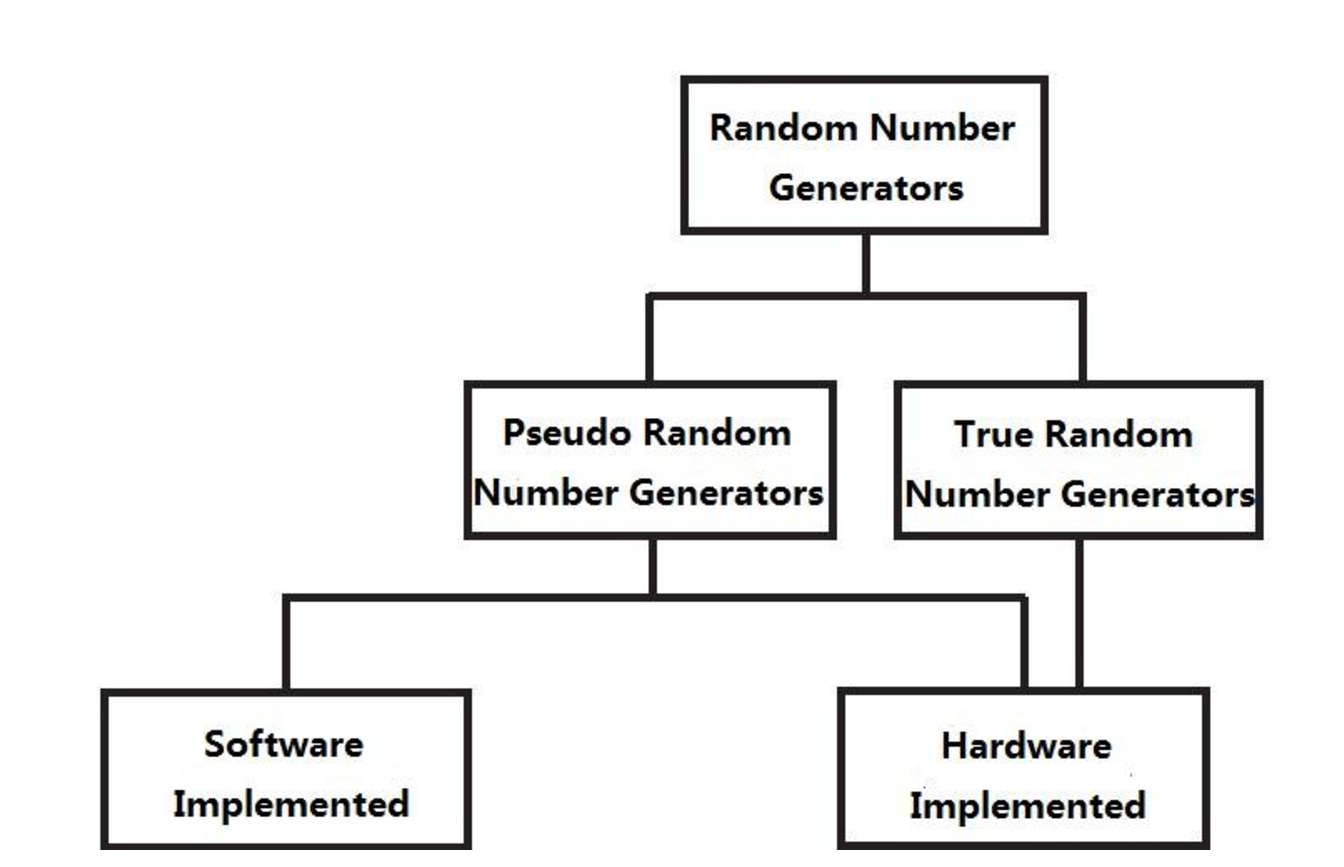
\includegraphics[width=3.85in]{Classification.eps}
\DeclareGraphicsExtensions.
\caption{Classification of random number generators}
\label{Classification}
\end{figure}



\subsection{True Random Number Generators (TRNGs)}
A TRNG is a physical device that generates statistically independent and unbiased bits. They are also
called non-deterministic RNGs. Such devices, which
exist too in computers, are often based on microscopic phenomena that generate a low-level, statistically random ``noise'' signal, such as thermal noise, photoelectric effect, or any other quantum phenomena. These processes are, in theory, completely unpredictable, and the theory's assertions of unpredictability are subject to experimental test. 

A quantum-based hardware random number generator typically consists in a transducer that converts some aspect of a given physical phenomena, into an electrical signal. An amplifier and other electronic circuitry bring the output of the transducer into the macroscopic realm, and some analog to digital converter translates the output into a digital number, often a simple binary digit 0 or 1. By repeatedly sampling the randomly varying signal, a series of random numbers is thus obtained.

\subsection{Pseudo Random Number Generators (PRNGs)}

A pseudorandom number generator (PRNG), also known as deterministic random bit generator (DRBG), is an algorithm for generating a sequence of numbers that approximates the properties of random numbers~\cite{Barker05recommendationfor}. The sequence is not truly random in that it is completely determined by a relatively small set of initial values, called the PRNG's state. Although sequences that are closer to truly random can be generated using hardware random number generators, pseudorandom numbers are important in practice for simulations (e.g., of physical systems with the Monte Carlo method), and are central in   cryptography and procedural generation due to their fundamental property of reproductibility. 

Common classes of these algorithms are linear congruential generators, Lagged Fibonacci generators, linear feedback shift registers, feedback with carry shift registers, and generalized feedback shift registers. Recent instances of pseudorandom algorithms include Blum Blum Shub, Fortuna, and the Mersenne twister.
All these generators will be developed later in this manuscript.

%\section{Cryptographically secure pseudo random number generators}
%
%
%A PRNG suitable for cryptographic applications is called a cryptographically secure PRNG (CSPRNG). A requirement for a CSPRNG is that an adversary not knowing the seed has only negligible advantage in distinguishing the generator's output sequence from a random sequence. In other words, while a PRNG is only required to pass certain statistical tests, a CSPRNG must pass all statistical tests that are restricted to polynomial time in the size of the seed. Though such property cannot be proven, strong evidence may be provided by reducing the CSPRNG to a known hard problem in mathematics (e.g., integer factorization). In general, years of review may be required before an algorithm can be certified as a CSPRNG.
%
%Some classes of CSPRNGs include the following:
%\begin{itemize}
%
%\item     Stream ciphers
%\item     Block ciphers running in counter or output feedback mode.
%\item     PRNGs that have been designed specifically to be cryptographically secure, such as Microsoft's Cryptographic 
% Application Programming Interface function CryptGenRandom, the Yarrow algorithm (incorporated in Mac OS X and FreeBSD), and Fortuna.
%\item     Combination PRNGs which attempt to combine several PRNG primitive algorithms with the goal of removing any non-randomness.
%\item     Special designs based on mathematical hardness assumptions. Examples include Micali-Schnorr and the Blum Blum Shub algorithm, which provide a strong security proof. Such algorithms are rather slow compared to traditional constructions, and impractical for many applications.
% 
%\end{itemize}

%\section{Stream Cipher}
%A stream cipher generates successive elements of the keystream based on an internal state. This state is updated in essentially two ways: if the state changes independently of the plaintext or ciphertext messages, the cipher is classified as a synchronous stream cipher. By contrast, self-synchronising stream ciphers update their state based on previous ciphertext digits.
%
%\subsection{One-Time Pad (Vernam Cipher)}
%In modern terminology, a Vernam cipher is a stream cipher in which the plaintext is XORed with a random or pseudorandom stream of data (the keystream) of the same length to generate the ciphertext. If the keystream is truly random and used only once, this is effectively a one-time pad. 
%
%Shannon~\cite{shannon-otp} showed that the one-time pad provides perfect security. This means
%that the conditional entropy of the message $M$ knowing the ciphertext $C$ is the same as the
%entropy of the original message, i.e. $H(M|C) = H(M)$. He also showed that the one-time
%pad is optimal in the sense that the previous conditions cannot be achieved with a key of
%size smaller than the message.
%
%The problem of the one-time pad is that we first have to agree on a key of the same
%length as the message. For most applications this is not practical. The next two schemes
%try to produce a ``random looking`` keystream from a short key and IV. By random looking,
%we mean that we cannot distinguish the keystream from a random sequence in a complexity
%less than trying all possible keys.
%
%\subsection{Synchronous stream ciphers}
%In a synchronous stream cipher a stream of pseudorandom digits is generated independently of the plaintext and ciphertext messages, and then combined with the plaintext (to encrypt) or the ciphertext (to decrypt). In the most common form, binary digits are used (bits), and the keystream is combined with the plaintext using the exclusive or operation (XOR). This is termed a binary additive stream cipher.
%
%In a synchronous stream cipher, the sender and receiver must be exactly in step for decryption to be successful. If digits are added or removed from the message during transmission, synchronisation is lost. To restore synchronisation, various offsets can be tried systematically to obtain the correct decryption. Another approach is to tag the ciphertext with markers at regular points in the output.
%
%If, however, a digit is corrupted in transmission, rather than added or lost, only a single digit in the plaintext is affected and the error does not propagate to other parts of the message. This property is useful when the transmission error rate is high; however, it makes it less likely the error would be detected without further mechanisms. Moreover, because of this property, synchronous stream ciphers are very susceptible to active attacks -- if an attacker can change a digit in the ciphertext, he might be able to make predictable changes to the corresponding plaintext bit; for example, flipping a bit in the ciphertext causes the same bit to be flipped in the plaintext.
%
%\subsection{Self-synchronizing stream ciphers}
%Another approach uses several of the previous N ciphertext digits to compute the keystream. Such schemes are known as self-synchronizing stream ciphers, asynchronous stream ciphers or ciphertext autokey (CTAK). The idea of self-synchronization was patented in 1946, and has the advantage that the receiver will automatically synchronise with the keystream generator after receiving N ciphertext digits, making it easier to recover if digits are dropped or added to the message stream. Single-digit errors are limited in their effect, affecting only up to N plaintext digits.
%
%An example of a self-synchronising stream cipher is a block cipher in cipher feedback (CFB) mode.
%


\subsection{Chaos-based Random Number Generators}

Since the seventies in last century, the use of chaotic dynamics for the generation of random sequences has raised a lot of interests. It is clearly pointed out by some researchers that there exists a close relationship between chaos and randomness, and many works have been witnessed in the last two decades~\cite{Provenzale199231}.
To do so, chaotic dynamics are usually studied in two different domains, depending on whether the generator is an hardware or a software one.
\begin{itemize}
 \item Continuous time domain: chaotic dynamics generated by differential equations.
 \item Discrete time domain: recurrent sequences using chaotic maps.
\end{itemize}

Chaos possesses several distinct properties that can possibly give meaning to the desire to use such dynamics for generating pseudorandomness, namely: the sensitivity to initial conditions, the ergodicity, the wide band spectrum, and the unpredictable and random-like behavior of iterates.
Although it is still controversy to equate these properties with randomness and claim a chaos-based random number generator to be good enough, a lot of designs and applications, in particular related to communications securing, have been proposed.

Nowadays, it is common to use a chaotic map for pseudorandom number generation. Due to the recent design of electronic circuits for the realization of chaotic systems, it is also possible to generate the bit sequence by observing such dynamics, as a replacement of those physical random sources.

\section{Statistical Tests for Randomness}
\label{Some famous statistical tests of random number generators}

A theoretical proof for the randomness of a generator is impossible to give, as such proof requires first to mathematically define what is randomness. Therefore statistical inference based on observed sample sequences produced by the generator seems to be the best option. Considering the properties of binary
random sequences, various statistical tests can be designed to evaluate the assertion
that the sequence is generated by a perfectly random source. 
We have performed certain statistical tests for various CI PRNGs we proposed. These tests
include TestU01~\cite{Lecuyer2009}, NIST suite~\cite{ANDREW2008},
DieHARD battery of tests~\cite{Marsaglia1996}, and Comparative test parameters. For completeness and for reference, we give
in the following subsection a brief description of each of the
aforementioned tests.



\subsection{NIST statistical test suite}



Among the numerous standard tests for pseudo-randomness, a convincing way to show the randomness of the produced sequences is to confront them to the NIST (National Institute of Standards and Technology) Statistical Test, because it is an up-to-date test suite proposed by the Information Technology Laboratory (ITL). A new version of the Statistical Test Suite (Version 2.0) has been released in August 11, 2010.


The NIST test suite SP 800-22 is a statistical package consisting of 15 tests. They were developed to test the randomness of binary sequences produced by hardware or software based cryptographic PRNGs. These tests focus on a variety of different types of non-randomness that could exist in a sequence. 


For each statistical test, a set of $p-values$ (corresponding to the set of sequences) is produced. The interpretation of empirical results can be conducted in any number of ways. In this manuscript, the examination of the distribution of $p-values$ to check for uniformity ($p-value_{T}$) is used:
the distribution of $P-values$ is examined to ensure uniformity. 
Concretely, this demand is verified in an usual way as follows: if $p-value_{T} \geqslant 0.0001$, then the sequences can be considered to be uniformly distributed.

In our experiments, 100 sequences (s = 100), each with 1,000,000-bit long, are generated and tested. If the $p-value_{T}$ of any test is smaller than 0.0001, the sequences are considered to be not good enough and the generating algorithm is not suitable for usage.

In what follows, the fifteen tests of the NIST Statistical tests suite, are recalled. A more detailed description for those tests could be found in \cite{ANDREW2008}.
\begin{itemize}
\item \textbf{Frequency (Monobit) Test (FT)} is to determine whether the number of ones and zeros in a sequence are approximately the same as would be expected for a truly random sequence.


\item \textbf{Frequency Test within a Block (FBT)} is to determine whether the frequency of ones in an M-bit block is approximately $M/2$, as would be expected under an assumption of randomness. %($M$ is the length of each block.)


\item \textbf{Runs Test (RT)} is to determine whether the number of runs of ones and zeros of various lengths is as expected for a random sequence. In particular, this test determines whether the oscillation between such zeros and ones is too fast or too slow.


\item \textbf{Test for the Longest Run of Ones in a Block (LROBT)} is to determine whether the length of the longest run of ones within the tested sequence is consistent with the length of the longest run of ones that would be expected in a random sequence.


\item \textbf{Binary Matrix Rank Test (BMRT)} is to check for linear dependence among fixed length substrings of the original sequence.


\item \textbf{Discrete Fourier Transform (Spectral) Test (DFTT)} is to detect periodic features (i.e., repetitive patterns that are near each other) in the tested sequence that would indicate a deviation from the assumption of randomness.


\item \textbf{Non-overlapping Template Matching Test (NOTMT)} is to detect generators that produce too many occurrences of a given non-periodic (aperiodic) pattern.


\item \textbf{Overlapping Template Matching Test (OTMT)} is to check the number of occurrences of pre-specified target strings.

\item \textbf{Maurer's ``Universal Statistical'' Test (MUST)} is to detect whether or not the sequence can be
significantly compressed without loss of information.

\item \textbf{Linear Complexity Test (LCT)} is to determine whether or not the sequence is complex enough to be considered random.

\item \textbf{Serial Test (ST)} is to determine whether the number of occurrences of the $2^{m}$ $m$-bit
overlapping patterns is approximately the same as would be expected for a random sequence.

\item \textbf{Approximate Entropy Test (AET)} is to compare the frequency of overlapping blocks of two consecutive/adjacent lengths (m and m+1) against the expected result for a random sequence.%(m is the length of each block.)

\item \textbf{Cumulative Sums (Cusum) Test (CST)} is to determine whether the cumulative sum of the partial sequences occurring in the tested sequence is too large or too small relative to the expected behavior of that cumulative sum for random sequences.

\item \textbf{Random Excursions Test (RET)} is to determine if the number of visits to a particular state within a cycle deviates from what one would expect for a random
sequence.

\item \textbf{Random Excursions Variant Test (REVT)} is to detect deviations from the expected number
of visits to various states in the random walk.
\end{itemize}

\subsection{DieHARD battery of tests}
The DieHARD battery of tests was developed in 1996 by Prof. Georges Marsaglia
from the Florida State University for testing randomness of sequences of numbers \cite{Marsaglia1996}. 
It has been the most sophisticated standard for over a decade. Because of the stringent requirements in the DieHARD test suite, a generator passing DieHARD battery of 
tests can be considered good as a rule of thumb. It was supposed to give a better way of analysis in comparison to original FIPS statistical tests.

The DieHARD battery of tests consists of 18 different independent statistical tests. 
Each test requires binary file of about 10-12 million bytes in order to run the full set of tests. 
As the NIST test suite, most of the tests in DieHARD return a $p-value$, which should be uniform on $[0,1)$ if the input file 
contains truly independent random bits. Those $p-values$ are obtained by
$p=F(X)$, where $F$ is the assumed distribution of the sample random variable $X$ (often normal). 
But that assumed $F$ is just an asymptotic approximation, for which the fit will be worst 
in the tails. Thus occasional $p-value$s near 0 or 1, such as 0.0012 or 0.9983 can occur. Unlike the NIST test suite, the test is considered to be successful when
the $p-value$ is in range $[0 + \alpha , 1 -\alpha ]$,
where $\sqrt{\alpha}$ is the level of significance of the test.

For example, with a level of significance of $5\%$, $p-values$ are expected to be in
$[0.025, 0.975]$. Note that if the $p-value$ is not in this range, it means that the null
hypothesis for randomness is rejected even if the sequence is truly random. These
tests are:
\begin{itemize}
\item \textbf{Birthday Spacings.} Choose random points on a large interval. The spacings
between the points should be asymptotically Poisson distributed. The name
is based on the birthday paradox.
\item \textbf{Overlapping Permutations.} Analyze sequences of five consecutive random
numbers. The 120 possible orderings should occur with statistically equal
probability
\item \textbf{Ranks of matrices.} Select some number
of bits from some number of random numbers to form a matrix over 0,1, then
determine the rank of the matrix. Count the ranks.
\item \textbf{Monkey Tests.} Treat sequences of some number of bits as ``words''. Count
the overlapping words in a stream. The number of ``words'' that don't appear
should follow a known distribution. The name is based on the infinite monkey
theorem.
\item \textbf{Count the 1's.} Count the 1 bits in each of either successive
or chosen bytes. Convert the counts to ``letters'', and count the occurrences
of five-letter ``words''
\item \textbf{Parking Lot Test.} Randomly place unit circles in a $100 \times 100 $ square. If the
circle overlaps an existing one, try again. After 12,000 tries, the number of
successfully ``parked'' circles should follow a certain normal distribution.
\item \textbf{Minimum Distance Test.} Randomly place 8,000 points in a $10,000 \times 10,000$ 
square, then find the minimum distance between the pairs. The square of this
distance should be exponentially distributed with a certain mean.
\item \textbf{Random Spheres Test.} Randomly choose 4,000 points in a cube of edge 1,000.
Center a sphere on each point, whose radius is the minimum distance to another point. The smallest sphere's volume should be exponentially distributed
with a certain mean.
\item \textbf{The Sqeeze Test.} Multiply 231 by random floats on [0,1) until you reach 1.
Repeat this 100,000 times. The number of floats needed to reach 1 should
follow a certain distribution.
\item \textbf{Overlapping Sums Test.} Generate a long sequence of random floats on [0,1).
Add sequences of 100 consecutive floats. The sums should be normally distributed with characteristic mean and sigma.
\item \textbf{Runs Test.} Generate a long sequence of random floats on [0,1). Count ascending and descending runs. The counts should follow a certain distribution.
\item \textbf{The Craps Test.} Play 200,000 games of craps, counting the wins and the number
of throws per game. Each count should follow a certain distribution.
\end{itemize}

\subsection{ENT test program}
%
ENT test program applies various tests to sequences of bytes stored in
files and reports the results of those tests. The program is useful
for evaluating random number generators for encryption and statistical
sampling applications, compression algorithms, and other applications
where the information density of a file is of interest~\cite{ent}.

There are 5 tests contained in the program:
%
\begin{enumerate}
\item Entropy test: Entropy testing, in bits per character (or byte), which
  corresponds to the incompressibility of the sequence (as a perfectly
  random sequence cannot be compressed, since no part of it can be
  expressed in terms of other parts). Hence entropy of 8 bits/byte
  means perfect randomness in the sense of incompressibility.
\item $\chi^2$ test: $\chi^2$ testing is very common for
  goodness-of-fit of sample distributions of random numbers. It is
  known to be very sensitive to deficiencies in random number
  generators (when it is located between 5\% to 95\%, data are treated
  as random).
\item Sample test: Sample test means can be tested for bias in random
  number generation. In binary mode, the expected mean is 0.5 while
  for bytes, the expected mean is 127.5.
\item Monte Carlo test: a Monte Carlo approximation of $\pi$, which is
  simply the evaluation the area of the unit circle using the $N$
  generated random numbers ($X_i$,$X_{i-1}$), $i = 2,...,N$.
\item Serial Correlation test: Serial correlation coefficient
  evaluated from $<X_i,X_{i-1}>/<X_i,X_i>$, for $i=2,..N$. The
  intended value for perfect random sequences is 0.
\end{enumerate}

\subsection{Comparative test parameters}

In this section, five well-known statistical tests~\cite{Menezes1997} are presented to play the role of easily verifiable comparison tools. They encompass frequency and autocorrelation tests. In what follows, $s = s^0,s^1,s^2,\dots , s^{n-1}$ denotes a binary sequence of length $n$. The question is to determine whether this sequence possesses some specific characteristics that a truly random sequence would be likely to exhibit. 


\paragraph{Frequency test (monobit test)}

The purpose of this test is to check if the numbers of 0's and 1's are approximately equal in $s$, as it would be expected for a random sequence. Let $n_0, n_1$ denote these numbers. The statistic used here is 
\begin{equation*}
X_1=\frac{(n_0-n_1)^2}{n}, 
\end{equation*}
which approximately follows a $\chi^2$ distribution with one degree of freedom when $n\geqslant 10^7$.

\paragraph{Serial test (2-bit test)}

The purpose of this test is to determine if the number of occurrences of 00, 01, 10, and 11 as subsequences of $s$ are approximately the same. Let $n_{00} , n_{01} ,n_{10}$, and $n_{11}$ denote the number of occurrences of $00, 01, 10$, and $11$ respectively. Note that $n_{00} + n_{01} + n_{10} + n_{11} = n-1$ since the subsequences are allowed to overlap. The
statistic used here is:
\begin{equation*}
X_2=\frac{4}{n-1}(n_{00}^2+n_{01}^2+n_{10}^2+n_{11}^2)-\frac{2}{n}(n_0^2+n_1^2)+1,
\end{equation*}
 which approximately follows a $\chi^2$ distribution with 2 degrees of freedom if $n\geqslant 21$.

\paragraph{Poker test}

The poker test studies if each pattern of length $m$ (without overlapping) appears the same number of times in $s$. Let $\lfloor \frac{n}{m} \rfloor\geqslant 5 \times 2^m$ and $k= \lfloor \frac{n}{m} \rfloor $. Divide the sequence $s$ into $k$ non-overlapping parts, each of length $m$. Let $n_i$ be the number of occurrences of the $i^{th}$ type of sequence of length $m$, where $1 \leqslant i \leqslant 2^m$. The statistic used is 
\begin{equation*}
X_3=\dfrac{2^m}{k}\left(\displaystyle{\sum^{2^m}_{i=1}n^2_i}\right)-k,
\end{equation*}
which approximately follows a $\chi^2$ distribution with $2^m-1$ degrees of freedom. Note that the poker test is a generalization of the frequency test (setting $m = 1$ in the poker test yields the frequency test).

\paragraph{Runs test}

The purpose of the runs test is to figure out whether the number of runs of various lengths in the sequence $s$ is as expected, for a random sequence. A run is defined as a pattern of all zeros or all ones, a block is a run of ones, and a gap is a run of zeros. The expected number of gaps (or blocks) of length $i$ in a random sequence of length $n$ is $e_i = \frac{n-i+3}{2^{i+2}}$. Let $k$ be equal to the largest integer $i$ such that $e_i \geqslant 5$. Let
$B_i , G_i$ be the number of blocks and gaps of length $i$ in $s$, for each $i \in \llbracket 1, k\rrbracket$. The statistic used here will then be:
\begin{equation*}
\displaystyle{X_4=\sum^k_{i=1}\frac{(B_i-e_i)^2}{e_i}+\sum^k_{i=1}\frac{(G_i-e_i)^2}{e_i}},
\end{equation*}
\noindent which approximately follows a $\chi^2$ distribution with $2k - 2$ degrees of freedom.

\paragraph{Autocorrelation test}

The purpose of this test is to check for coincidences between the sequence $s$ and (non-cyclic) shifted versions of it. Let $d$ be a fixed integer, $ 1 \leqslant d \leqslant \lfloor n/2 \rfloor$. The value $A(d) = \sum_{i=0}^{n-d-1} s_i\oplus s_{i+d}$ is the amount of bits not equal between the sequence and itself displaced by $d$ bits. The statistic used is:
\begin{equation*}
X_5=\dfrac{2 \left(A(d)-\frac{n-d}{2}\right)}{\sqrt{n-d}},
\end{equation*}
which approximately follows a normal distribution $\mathcal{N}(0, 1)$ if $n-d \geqslant 10$. Since small values of $A(d)$ are as unexpected as large values, a two-sided test should be used.

\subsection{TestU01 Statistical Test}
\label{Testing a generator}

TestU01 is extremely diverse in implementing classical tests,
cryptographic tests, new tests proposed in the literature, and original tests.
In fact, it encompasses most of the other testsuites. 
There are seven batteries of tests in the TestU01 package, which are listed in what follows:

\begin{itemize}
\item{\textbf{SmallCrush.}} The first battery to check, with 15 $p-$values reported. This is a fast collection of tests used to be sure that the basic requirements of randomness are satisfied. In case of success, this battery should be followed by Crush and BigCrush.
\item{\textbf{Crush.}} This battery includes many difficult tests, like those described in~\cite{Knuth1998}. %Cette référence n'apparaît pas.
%D. E. Knuth. The Art of Computer Programming, Volume 2: Seminumerical Algorithms. Addison-Wesley, Reading, Mass., third edition, 1998.
It uses approximately $2^{35}$ random numbers and applies 96 statistical tests
(it computes a total of 144 test statistics and $p-values$).
\item{\textbf{BigCrush.}} The BigCrush uses
approximately $2^{38}$ random numbers and applies 106 tests (it computes 160 test
statistics and $p-values$). 
A suite of very stringent statistical tests, and the most difficult battery to pass.
\item{\textbf{Rabbit.}} This battery of tests reports 38 $p-values$.
\item{\textbf{Alphabit.}} Alphabit and AlphabitFile have been designed primarily to test hardware random bits generators. 17 $p-values$ are reported here.
\item{\textbf{Pseudo-DieHARD.}} This battery implements most of the tests contained in the popular battery DieHARD or, in some cases, close approximations to them. It is not a very stringent battery. Indeed, there is no generator that can pass Crush and BigCrush batteries and fail Pseudo-DieHARD, while the converse occurs for several defective generators. 126 $p-values$ are reported here.
\item{\textbf{FIPS\_140\_2.}} As recalled previously, the NIST (National Institute of Standards and Technology) of the U.S. federal government has proposed a statistical test suite. It is used to evaluate the randomness of bitstreams produced by cryptographic random number generators. This battery reports 16 $p-values$.
\end{itemize}

Six predefined batteries of tests are available in TestU01; three of them
are for sequences of $\mathcal{U}(0, 1)$ random numbers and the three others are for bit
sequences. In the first category, we have SmallCrush, Crush, and BigCrush.

To test a RNG for general use,
one could first apply the small and fast battery SmallCrush. If it passes, one could then apply
the more stringent battery Crush, and finally the yet more time-consuming battery BigCrush.
These batteries of tests include the classical tests described in Knuth~\cite{Knuth1998}, for
example: the run, poker, coupon collector, gap, max-of-t, and permutation tests.
There are collision and birthday spacings tests in 2, 3, 4, 7, 8 dimensions, several close pairs tests in 2, 3, 5, 7, 9 dimensions, and correlation tests. Some
tests use the generated numbers as a sequence of ``random'' bits: random walk
tests, linear complexity tests, a Lempel-Ziv compression test, several Hamming
weights tests, matrix rank tests, run and correlation tests, among others.




The batteries Rabbit, Alphabit, and BlockAlphabit are for binary sequences
(e.g., a cryptographic pseudorandom generator or a source of random bits
produced by a physical device). They were originally designed to test a finite
sequence contained in a binary file. When invoking the battery, one must specify the number $n_B$ of bits available for each test. When the bits are in a file, $n_B$
must not exceed the number of bits in the file, and each test will reuse the same
sequence of bits starting from the beginning of the file (so the tests are not independent). When the bits are produced by a generator, each test uses a different
stream. In both cases, the parameters of each test are chosen automatically as
a function of $n_B$ .
The batteries Alphabit and Rabbit can be applied on a binary file considered as a source
of random bits. They can also be applied on a programmed generator. Alphabit has been
defined primarily to test hardware random bits generators. The battery PseudoDieHARD
applies most of the tests in the well-known DieHARD suite of Marsaglia [106]. The battery
FIPS\_140\_2 implements the small suite of tests of the FIPS\_140\_2 standard from NIST.
The batteries described in this module will write the results of each test (on standard
output) with a standard level of details (assuming that the Boolean switches of module
swrite have their default values), followed by a summary report of the suspect p-values
obtained from the specific tests included in the batteries. It is also possible to get only the
summary report in the output, with no detailed output from the tests, by setting the Boolean
switch swrite\_Basic to FALSE. Rabbit and Alphabit apply 38 and 17 different statistical tests,
respectively. 

Some of the tests compute more than one statistic (and $p-value$) using the same stream of random
numbers and these statistics are thus not independent. That is why the number of statistics
in the summary reports is larger than the number of tests in the description of the batteries.
For a more detailed description, the reader is referred
to the documentation of the TestU01 library.

\begin{itemize}
\item{\textbf{Small Crush:}}\\smarsa\_BirthdaySpacings \\ 
 sknuth\_Collision \\ 
 sknuth\_Gap\\ 
 sknuth\_SimpPoker \\ 
 sknuth\_CouponCollector\\ 
 sknuth\_MaxOft \\ 
 svaria\_WeightDistrib \\ 
 smarsa\_MatrixRank \\
 sstring\_HammingIndep\\ 
 swalk\_RandomWalk1\\ 
\item{\textbf{Crush:}}\\smarsa\_SerialOver \\
 smarsa\_CollisionOver\\ 
 smarsa\_BirthdaySpacings\\ 
 snpair\_ClosePairs\\ 
 snpair\_ClosePairsBitMatch \\
 sknuth\_SimpPoker\\ 
 sknuth\_CouponCollector\\ 
 sknuth\_Gap\\ 
 sknuth\_Run\\ 
 sknuth\_Permutation\\ 
 sknuth\_CollisionPermut\\ 
 sknuth\_MaxOft\\ 
 svaria\_SampleProd\\ 
 svaria\_SampleMean \\ 
 svaria\_SampleCorr\\ 
 svaria\_AppearanceSpacings \\
 svaria\_WeightDistrib \\
 svaria\_SumCollector\\ 
 smarsa\_MatrixRank\\ 
 smarsa\_Savir2\\ 
 smarsa\_GCD\\ 
 swalk\_RandomWalk1\\ 
 scomp\_LinearComp \\
 scomp\_LempelZiv\\ 
 sspectral\_Fourier3\\ 
 sstring\_LongestHeadRun \\
 sstring\_PeriodsInStrings\\ 
 sstring\_HammingWeight2\\ 
 sstring\_HammingCorr\\ 
 sstring\_HammingIndep \\
 sstring\_Run\\ 
 sstring\_AutoCor \\ 
\item{\textbf{Big Crush:}}\\smarsa\_SerialOver\\ 
smarsa\_CollisionOver\\ 
smarsa\_BirthdaySpacings\\ 
snpair\_ClosePairs \\ 
sknuth\_SimpPoker\\ 
sknuth\_CouponCollector\\ 
sknuth\_Gap\\ 
sknuth\_Run\\ 
sknuth\_Permutation\\ 
sknuth\_CollisionPermut\\ 
sknuth\_MaxOft\\ 
svaria\_SampleProd\\ 
svaria\_SampleMean\\ 
svaria\_SampleCorr\\ 
svaria\_AppearanceSpacings\\ 
svaria\_WeightDistrib\\ 
svaria\_SumCollector\\ 
smarsa\_MatrixRank\\ 
smarsa\_Savir2\\ 
smarsa\_GCD\\ 
swalk\_RandomWalk1\\ 
scomp\_LinearComp\\ 
scomp\_LempelZiv\\ 
sspectral\_Fourier3\\ 
sstring\_LongestHeadRun\\ 
sstring\_PeriodsInStrings\\ 
sstring\_HammingWeight2\\ 
sstring\_HammingCorr\\ 
sstring\_HammingIndep\\ 
sstring\_Run\\ 
sstring\_AutoCor\\ 

\item{\textbf{Rabbit:}}\\smultin\_MultinomialBitsOver\\ 
snpair\_ClosePairsBitMatch\\ 
svaria\_AppearanceSpacings\\ 
scomp\_LinearComp\\ 
scomp\_LempelZiv\\ 
sspectral\_Fourier1\\ 
sspectral\_Fourier3\\ 
sstring\_LongestHeadRun\\ 
sstring\_PeriodsInStrings\\ 
sstring\_HammingWeight\\ 
sstring\_HammingCorr\\ 
sstring\_HammingIndep\\ 
sstring\_AutoCor\\ 
sstring\_Run\\ 
smarsa\_MatrixRank\\ 
swalk\_RandomWalk1\\ 

\item{\textbf{Alphabit:}}\\smultin\_MultinomialBitsOver\\ 
sstring\_HammingIndep\\ 
sstring\_HammingCorr\\ 
swalk\_RandomWalk1 \\ 


\item{\textbf{Pseudo-DieHARD:}}\\Birthday Spacings test\\ 
Overlapping 5-Permutation test\\ 
Binary Rank Tests for Matrices test\\ 
Bitstream test\\ 
OPSO test\\ 
OQSO test\\ 
DNA test\\ 
Count-the-1's test\\ 
Parking Lot test\\ 
Minimum Distance test\\ 
3-D Spheres test\\ 
Squeeze test\\ 
Overlapping Sums test\\ 
Runs test\\ 
Craps test\\ 

\item{\textbf{FIPS\_140\_2:}}\\Monobit test\\ 
``poker'' test\\ 
Runs test\\ 
Longest Run of Ones in a Block test

\end{itemize}

TestU01 suite implements hundreds of tests and reports $p-$values. If a $p-$value is within $[0.001,0.999]$, the associated test is a success. A $p-$value lying outside this boundary means that its test has failed. %This is the standard range the test-suite suggests. The p-value selection criteria for the various test suites were chosen to produce a few failures in the best cases. Setting the criteria too low (closer to zero) would exhibit no failures and setting the criteria too high would fail everything.




\section{FPGA}
We finally introduce the field-programmable gate array (FPGA) architecture, on which our generators will be
implemented. 

A FPGA is an integrated circuit designed to be configured by a customer or a designer after manufacturing-hence ``field-programmable'' 
\begin{figure}
\centering
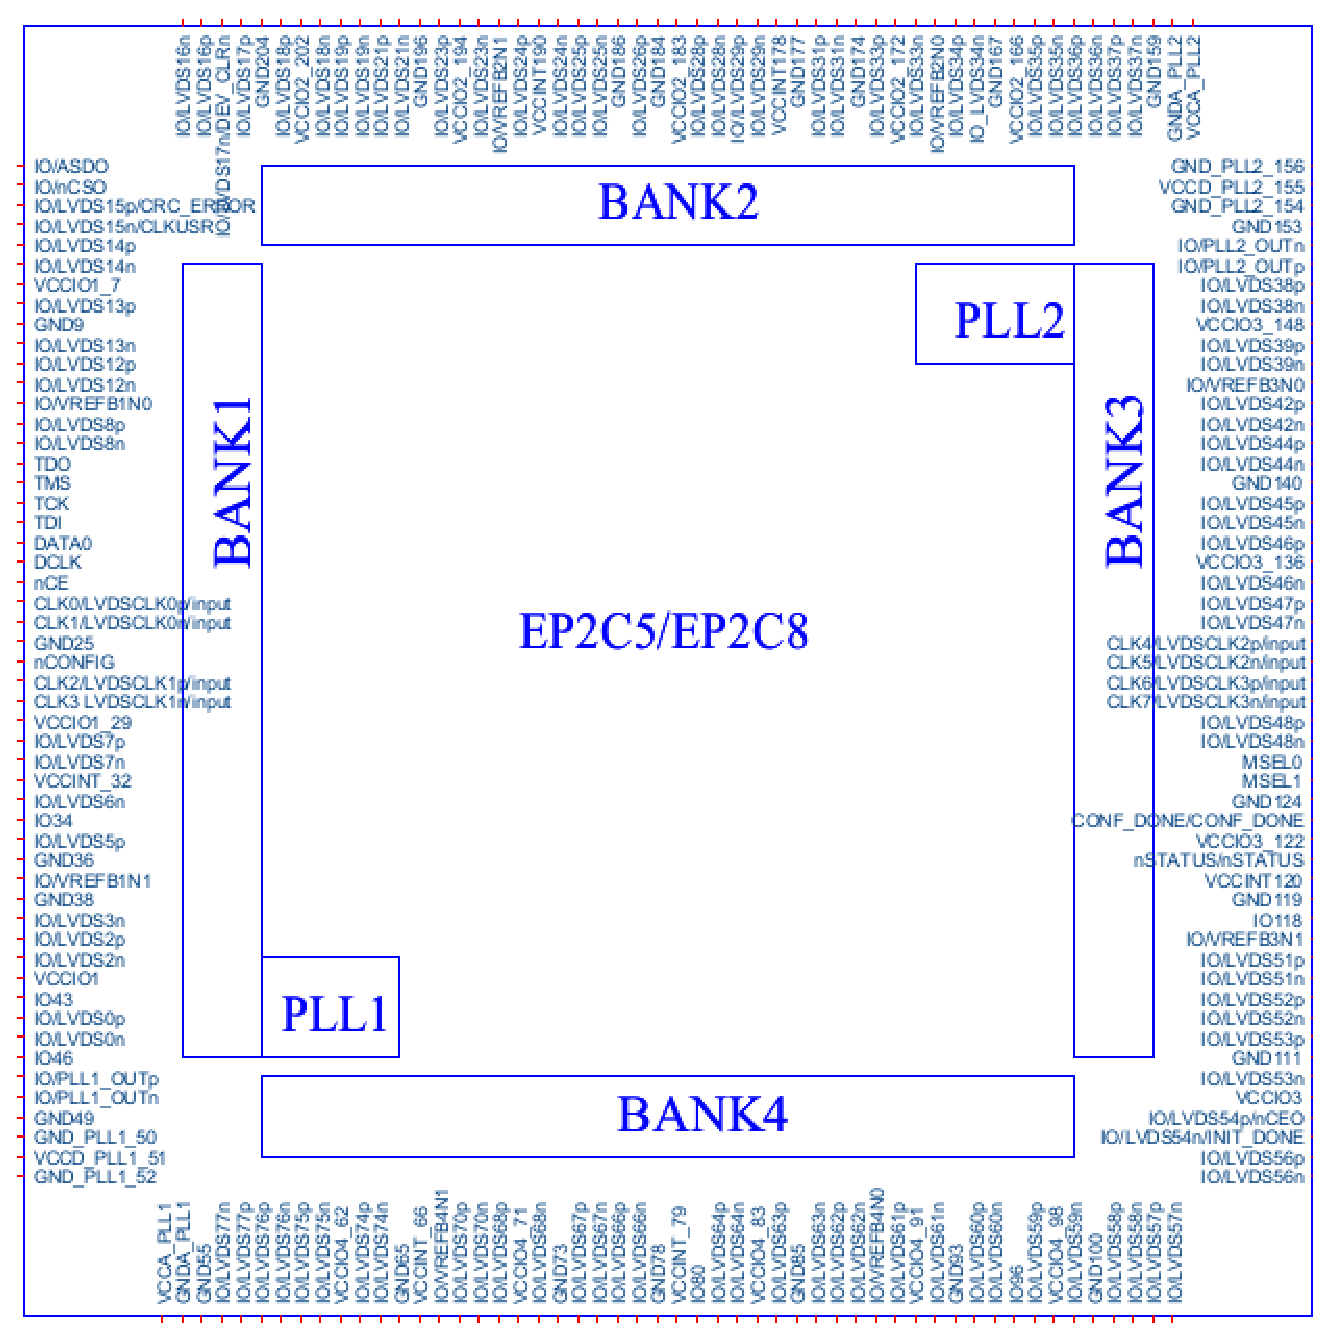
\includegraphics[width=5in]{fpga_scheme.eps}
\DeclareGraphicsExtensions.
\caption{FPGA EP2C8 core from ALTERA company}
\label{fpga_scheme}
\end{figure}
%The experiments in this research were implemented on FPGA. 
(a FPGA is indeed a VLSI chip with some special features).
The most common FPGA architecture consists of an array of logic blocks (called Configurable Logic Block, CLB, or Logic Array Block, LAB, depending on vendor), I/O pads, and routing channels. Generally, all the routing channels have the same width (number of wires). Multiple I/O pads may fit into the height of one row or the width of one column in the array. There are some primitives such as lookup tables (LUT) and flip-flop (FF) inside the CLB. The functions of these primitives and connections between them can be configured for different designs. Programmable routing matrices (PRM), implemented in static RAMs, are used to connect the I/O ports of the CLBs.

The advantages of FPGA designs over traditional VLSI designs are:
\begin{itemize}
\item The feasibility of reusing fast design to product time and chips for different designs.
\item Easy simulation and debugging. Software simulator and debugger provide
efficient methods of finding bugs and estimating of performance.
\item Low cost prototyping for early designs.
\item Design can be upgraded after deployment without hardware replacement.
\item Developing  hardware  systems  using  design  tools  for  FPGA  is  as  easy  as developing a software system.
\item FPGA can be reprogrammed on the field. 
\end{itemize}

To define the behavior of the FPGA, the user provides a hardware description language (HDL) or a schematic design. The most common HDLs are VHDL and Verilog, although in an attempt to reduce the complexity of designing in HDLs, which have been compared to the equivalent of assembly languages, there are moves to raise the abstraction level through the introduction of alternative languages. 

A general structure outline of FPGA core (EP2C8) used in this thesis is shown in Fig.\ref{fpga_scheme}


